% Chapter Template

\chapter{Methodology}

\label{Methodology}

\section{Dataset Selection}

As has been stated previously in this thesis, the dataset that is used in the analysis of this model is JHMDB \cite{JHMDB}. This dataset was selected for one primary reason, consistency when comparing one model to another. As was discussed in section \ref{sec:pose-detection}, typical pose-based action recognition models utilize a two-step approach which involves first extracting pose data, then using that pose data in order to build intermediate representations. Usage of this dataset standardizes this first step since the pose data is included, rather than needing to be generated by a separate model. This means that a more direct comparison can be drawn from other models since the input data is all the same. It is an understood fact throughout the remainder of this thesis that small gains may be able to be made through the addition of a more accurate pose model, however the scope of this thesis specifically focuses on the intermediate representation and corresponding models that process this representation.

\section{Pose}

The methodology throughout this section is dependent on pose information output from models that were described in section \ref{sec:pose-detection}. These pose models have several outputs used by similar models such as joint heatmaps, however the main focus of this paper is the positions of the joints. These joints can be connected by lines to form "bones" which are then all connected together to form a "skeleton". This skeleton is shown in figure \ref{fig:pose}, where each of the joints are connected to form a human-like figure that can easily be created form the x \& y coordinates of the joints.

\begin{figure}[ht]
	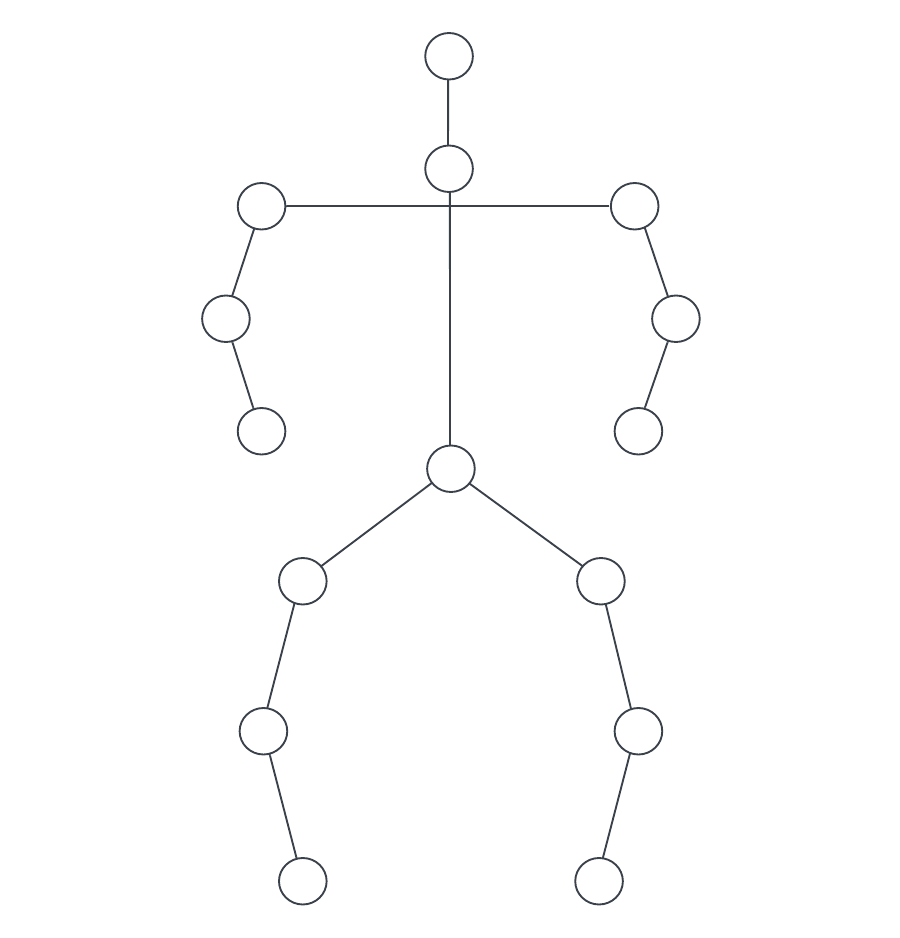
\includegraphics[width=0.5\textwidth]{pose}
	\centering
	\caption{Example of how joints are connected through bones in a typical pose representations.}
	\label{fig:pose}
\end{figure}

Using the JHMDB dataset, we simply take the existing pose implementation, the representation and indexes being shown in figure \ref{fig:JHMDB}, with 15 total joints. Specifically in this thesis, we are concerned with bone-joint-bone connections, effectively representing the angle of the middle joint and how the bones around it move.

\subsection{Joint Angles}

The core of how the new representation will represent actions and movement has to do with the angle between two bones at any one given joint.

\begin{figure}[ht]
	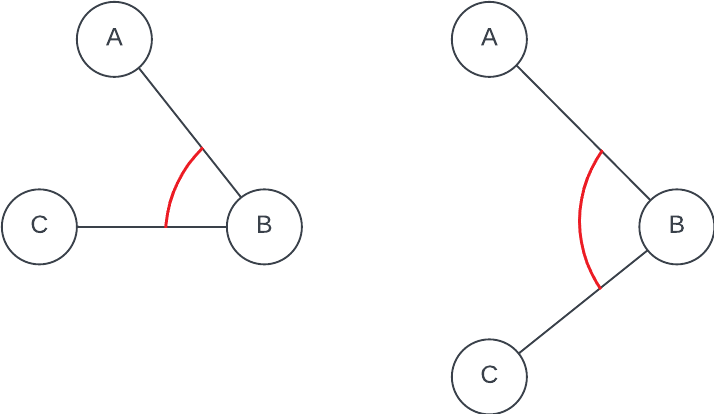
\includegraphics[width=0.8\textwidth]{JointAngles}
	\centering
	\caption{Two examples of three joints interconnected with two bones, and how the angle can change from one frame to another.}
	\label{fig:joint-angles}
\end{figure}

The first step in calculating the directional angle between the two vectors is to center one of the joints at the origin. Throughout this chapter, we will be referring to these two vectors as $a$ and $b$. In figure \ref{fig:joint-angles}, "$a$" would be denoting the vector $B \rightarrow A$ and "$b$" the vector $B \rightarrow C$. In this example, "$B$" will be the origin. This origin centering is simple and is done by the following equation \ref{eqn:angle-centering}, with each point representation as it was in figure \ref{fig:joint-angles} using the $B \rightarrow A$ bone as an example.

\begin{equation}
	\label{eqn:angle-centering}
	\centering
	a(x,y) = (A.x - B.x, A.y - B.y)
\end{equation}

After processing both bones through this equation, it produces two vectors beginning at the origin. The goal then becomes calculating the angle between two of these vectors. This can be easily done by leveraging arctan. Calculating the angle of a given vector '$a$' to the x-axis is simply done by using $\arctan(a.y/a.x)$. Once we have the angle of this vector to the x-axis, we can convert it to a positive value to ensure that the angle is being measured from a clockwise direction. Afterwards, we simply take the difference of the two vectors to determine the clockwise directional angle between two given vectors as denoted in equation \ref{eqn:angle-calculation}.

\begin{equation}
	\label{eqn:angle-calculation}
	\centering
	\arctan(a.y/a.x) - \arctan(b.y/b.x)
\end{equation}

The angle is calculated in a particular direction because if it were simply to be calculated agnostic of direction, it would be impossible to determine what angle a joint moves if it were to cross the $180^\circ$ boundary. Table \ref{tab:directed-angle-example} demonstrates this issue, where a $180^\circ$ rotation is observed from one right angle to another, but if non-directional angle is used, no change is represented. This prevents us from using a simpler solution such as the dot product to calculate these angles.

\begin{table}[ht]
	\centering
	\begin{tabular}{||c c c c||} 
		\hline
		\textbf{a(x,y)} & \textbf{b(x,y)} & \textbf{Directional} & \textbf{Non-Directional} \\ [0.5ex] 
		\hline\hline
		$(1,0)$ & $(0,1)$ & $90^\circ$ & $90^\circ$ \\
		\hline
		$(1,0)$ & $(0,-1)$ & $270^\circ$ & $90^\circ$ \\
		\hline
	\end{tabular}
	\caption{Example of how non-directional angle can result in incorrect rotation changes from one frame to another.}
	\label{tab:directed-angle-example}
\end{table}

The resulting method means that some angles will be measured from the "outside" of the person and some will be measured from the "inside" as shown in figure \ref{fig:pose-joint-angles}. In practice, this does not have a large effect on the representation as the primary factor in this method is the change of an angle from one frame to another which is indifferent to how the angle is measured as long as the distance is consistent.

\begin{figure}[ht]
	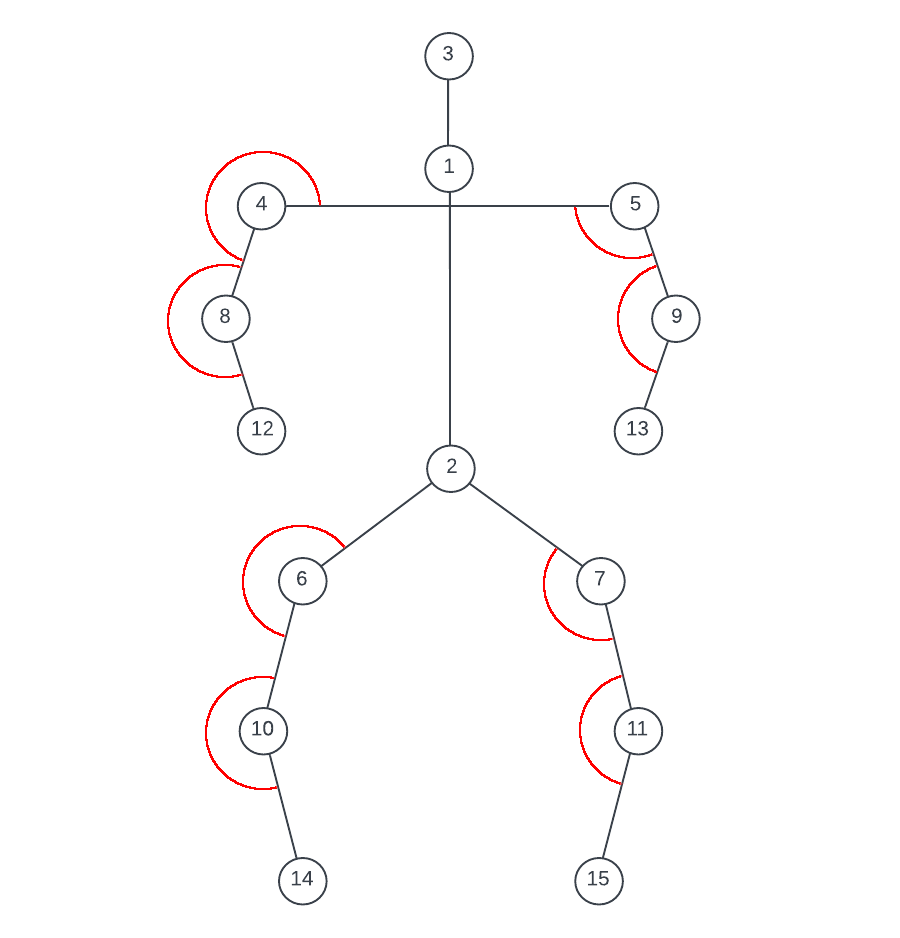
\includegraphics[width=5cm]{PoseJointAngles}
	\centering
	\caption{An example skeleton with JHMDB indices in each of the joints. In addition, angles have been shown as if they are being calculated in a clockwise direction, resulting in connections such as 5-4-8 having the angle on the "outside" of the person.}
	\label{fig:pose-joint-angles}
\end{figure}

\subsection{Joint Velocities}
\label{sec:joint-velocities}

Once the joint angles for each frame have been extracted, the next step before implementation into our representation is to determine the change of a joint angle from one frame to another to determine the "velocity" of said joint angle. Generally this is simply done by calculating $angle_2 - angle_1$, however there is one exception where the angle change crosses over the positive x-axis. This would be an example such as the difference between $angle_1 = 5$ and $angle_2 = 350$. The correct description would be that the angle moved $-15^\circ$, however using that simple calculation would mean that the model would interpret this as a $345^\circ$ change. This is most likely incorrect, as the more likely scenario is that the person moved $-15^\circ$ rather than almost a complete rotation in the other direction. So we add logic such that if the difference between two angles is greater than $180^\circ$ or lower than $-180^\circ$, the most likely scenario is that it moved in the opposite direction for a shorter distance. So a change such as $270^\circ$ would become $-90^\circ$ and similarly a change of $-270^\circ$ would become $90^\circ$.

\section{Novel Intermediate Representation}

We can now construct the indermediate representation that will be used as input to our model. The model representation is very similar to that in the \textbf{Simple yet efficient real-time pose-based action recognition} \cite{simple_yet_efficient} as described in section \ref{sec:intermediate}, which involves constructing a 2 dimensional image that is easily fed into a simple model. This is represented in figure \ref{fig:intermediate-construction}, where one joint angle is taken from one frame of the video, and added to a column. This column consists of all of the data for one frame of the video, which is then added to the rest of the representation, eventually constructing the joint angles for each frame of the video.

\begin{figure}[ht]
	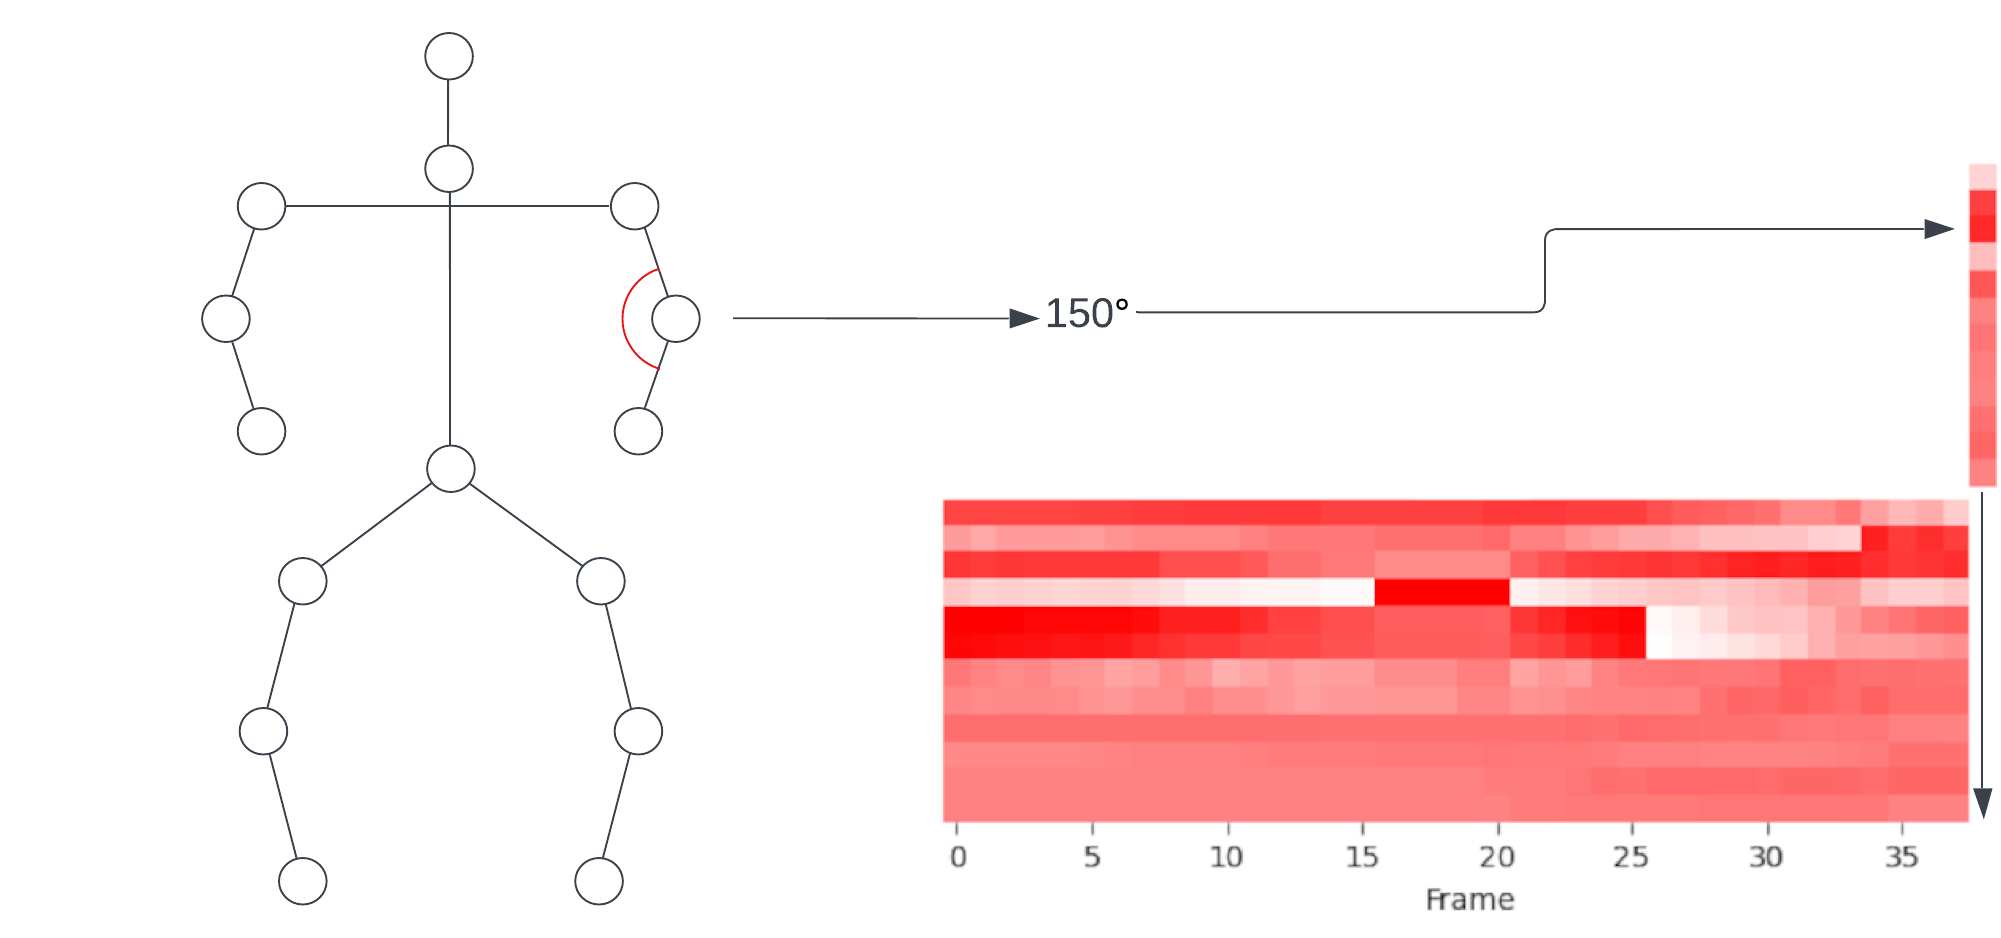
\includegraphics[width=\textwidth]{IntermediateConstruction}
	\centering
	\caption{Example of how the intermediate representation is constructed. At each frame, the angles of each joint are taken and added to a column, each column is then stacked next to one another to form a 2 dimensional image.}
	\label{fig:intermediate-construction}
\end{figure}

As described previously in section \ref{sec:joint-velocities}, a key point of our representation is the joint velocities portion. These values can simply be "stacked" on top of the angles to form the full intermediate representation. The logic is that for any given frame $i$, the column contains both the joint angles for the frame $i$, as well as their differences between frame $i$ and $i+1$, the completed representation shown in figure \ref{fig:intermediate-stacked}.

\begin{figure}[ht]
	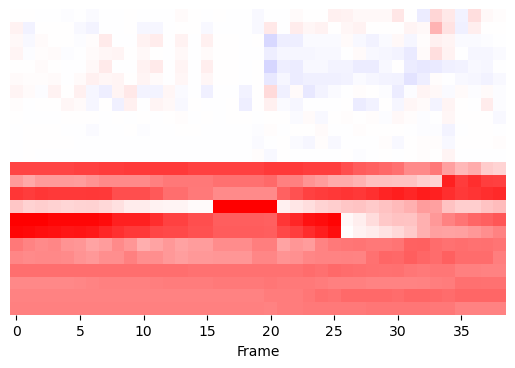
\includegraphics[width=8cm]{IntermediateStacked}
	\centering
	\caption{The completed intermediate representation, the top half contains the changes in joint angle from one frame to another (also referred to as "velocity"), and the bottom half contains the joint angles themselves. This is referred to as the "stacked" representation. In the representation, positive values are shown as red and negative values are shown as blue, with the higher values having more saturation.}
	\label{fig:intermediate-stacked}
\end{figure}

The specific joints that are represented in our intermediate representation are shown in table \ref{tab:joint-connections}. These joints were chosen as they are major joints that form the typical "skeleton" visualization similar to that shown in figure \ref{fig:pose} and \ref{fig:pose-joint-angles}.

\begin{table}[ht]
	\centering
	\begin{tabular}{||c c c c||} 
		\hline
		\textbf{Joint A} & \textbf{Joint B} & \textbf{Joint C} & \textbf{JHMDB Indices} \\ [0.5ex] 
		\hline\hline
		Face & Neck & Right Shoulder & $(3, 1, 4)$ \\
		Face & Neck & Left Shoulder & $(3, 1, 4)$ \\
		\hline
		Right Elbow & Right Shoulder & Left Shoulder & $(8, 4, 5)$ \\
		Left Elbow & Left Shoulder & Right Shoulder & $(9, 5, 4)$ \\
		\hline
		Right Elbow & Right Shoulder & Right Hip & $(8, 4, 6)$ \\
		Left Elbow & Left Shoulder & Left Hip & $(9, 5, 7)$ \\
		\hline
		Right Wrist & Right Elbow & Right Shoulder & $(12, 8, 4)$ \\
		Left Wrist & Left Elbow & Left Shoulder & $(13, 9, 5)$ \\
		\hline
		Right Shoulder & Right Hip & Right Knee & $(4, 6, 10)$ \\
		Left Shoulder & Left Hip & Left Knee & $(5, 7, 11)$ \\
		\hline
		Right Hip & Right Knee & Right Ankle & $(6, 10, 14)$ \\
		Left Hip & Left Knee & Left Ankle & $(7, 11, 15)$ \\
		\hline
	\end{tabular}
	\caption{All Joint connections used in our intermediate representations. The joint angle that is focused on is centered on the \textbf{B} joint, with the two vectors $B \rightarrow A$ and $B \rightarrow C$ forming the angle used in the representation.}
	\label{tab:joint-connections}
\end{table}

\subsection{Representation Features}

The way the representation is constructed results in a representation that is 2-D rotation invariant, scale invariant, and global position invariant, providing us with advantages over other models.

\textbf{Rotation} does not affect the representation since the angle of a joint from one frame to another only relies on the two bones, the two bones can rotate globally, what matters is only the angle between the two given bones. This effect is shown in figure \ref{fig:rotation-invariant}, where the angle of interest does not change when another joint next to it is rotated, this can be generalized to any global rotation with the same logic.

\begin{figure}[ht]
	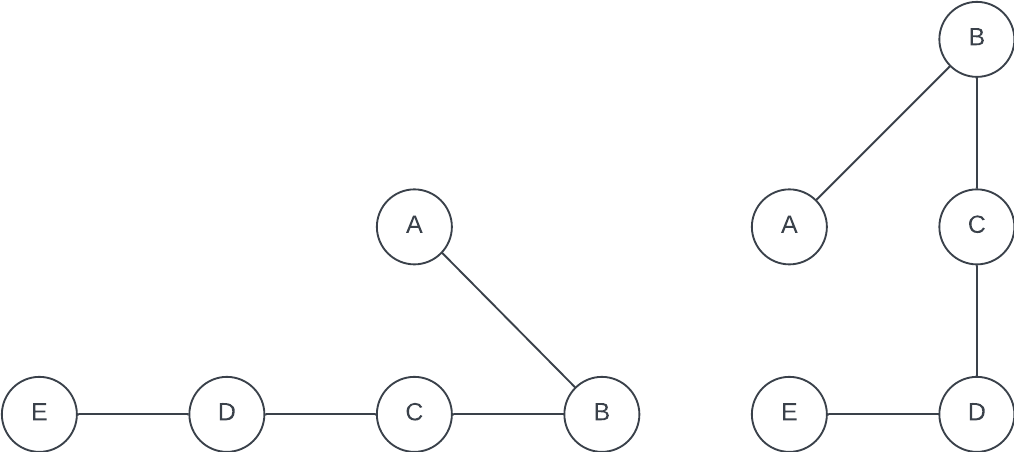
\includegraphics[width=0.8\textwidth]{RotationExample}
	\centering
	\caption{Example of the rotation invariance of our representation. The angle represented is $A-B-C$, and is unaffected by a rotation around $C-D-E$, remaining at $45^{\circ}$}.
	\label{fig:rotation-invariant}
\end{figure}

\textbf{Scale} is avoided entirely as we do not take into account the length of the bones, rather only the angle of the joints. As was stated previously in this chapter, the bones are converted to vectors prior to computing the angle between them. This involves normalizing both bones to be length one, and this length data is not held for any part of the representation. Therefore, the person can move closer or farther from the camera during the action, and it will have no effect on the representation.

\textbf{Global Position} is the final feature that the representation is invariant to. Similar to the previous features, the representation only cares about the angle of the specified joint, meaning that we can translate the person from one side of the frame to another with no change in the representation.

These three features of the model aim to mitigate background interference that has been previously discussed in the model. Specifically, they aim to reduce interference from movement of the camera. A person can move to either side, closer or farther away, and rotate the camera  and there will be no effect on the representation.

\subsection{Representation Comparison}

Comparing our representation to other intermediate representations, there are many similarities that can be observed.

The overall structure of the representation was largely inspired by \textbf{Simple yet efficient real-time pose-based action recognition} \cite{simple_yet_efficient}, as shown in figure \ref{fig:simple-v-ours}. While the construction of this 2 dimensional grid was a very efficient way to construct the representation, their representation relied on the cartesian coordinates, resulting in a representation more susceptible to background interference. However, the general structure of the image was adapted for our use, simply using a different data source (joint angles + velocities).

\begin{figure}[ht]
	\subfigure[]{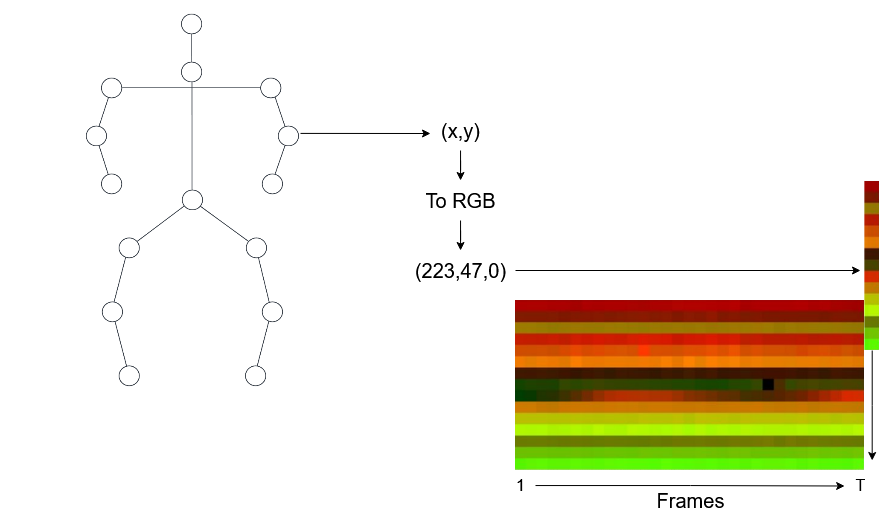
\includegraphics[width=0.6\textwidth]{EHPIv2}}
	\subfigure[]{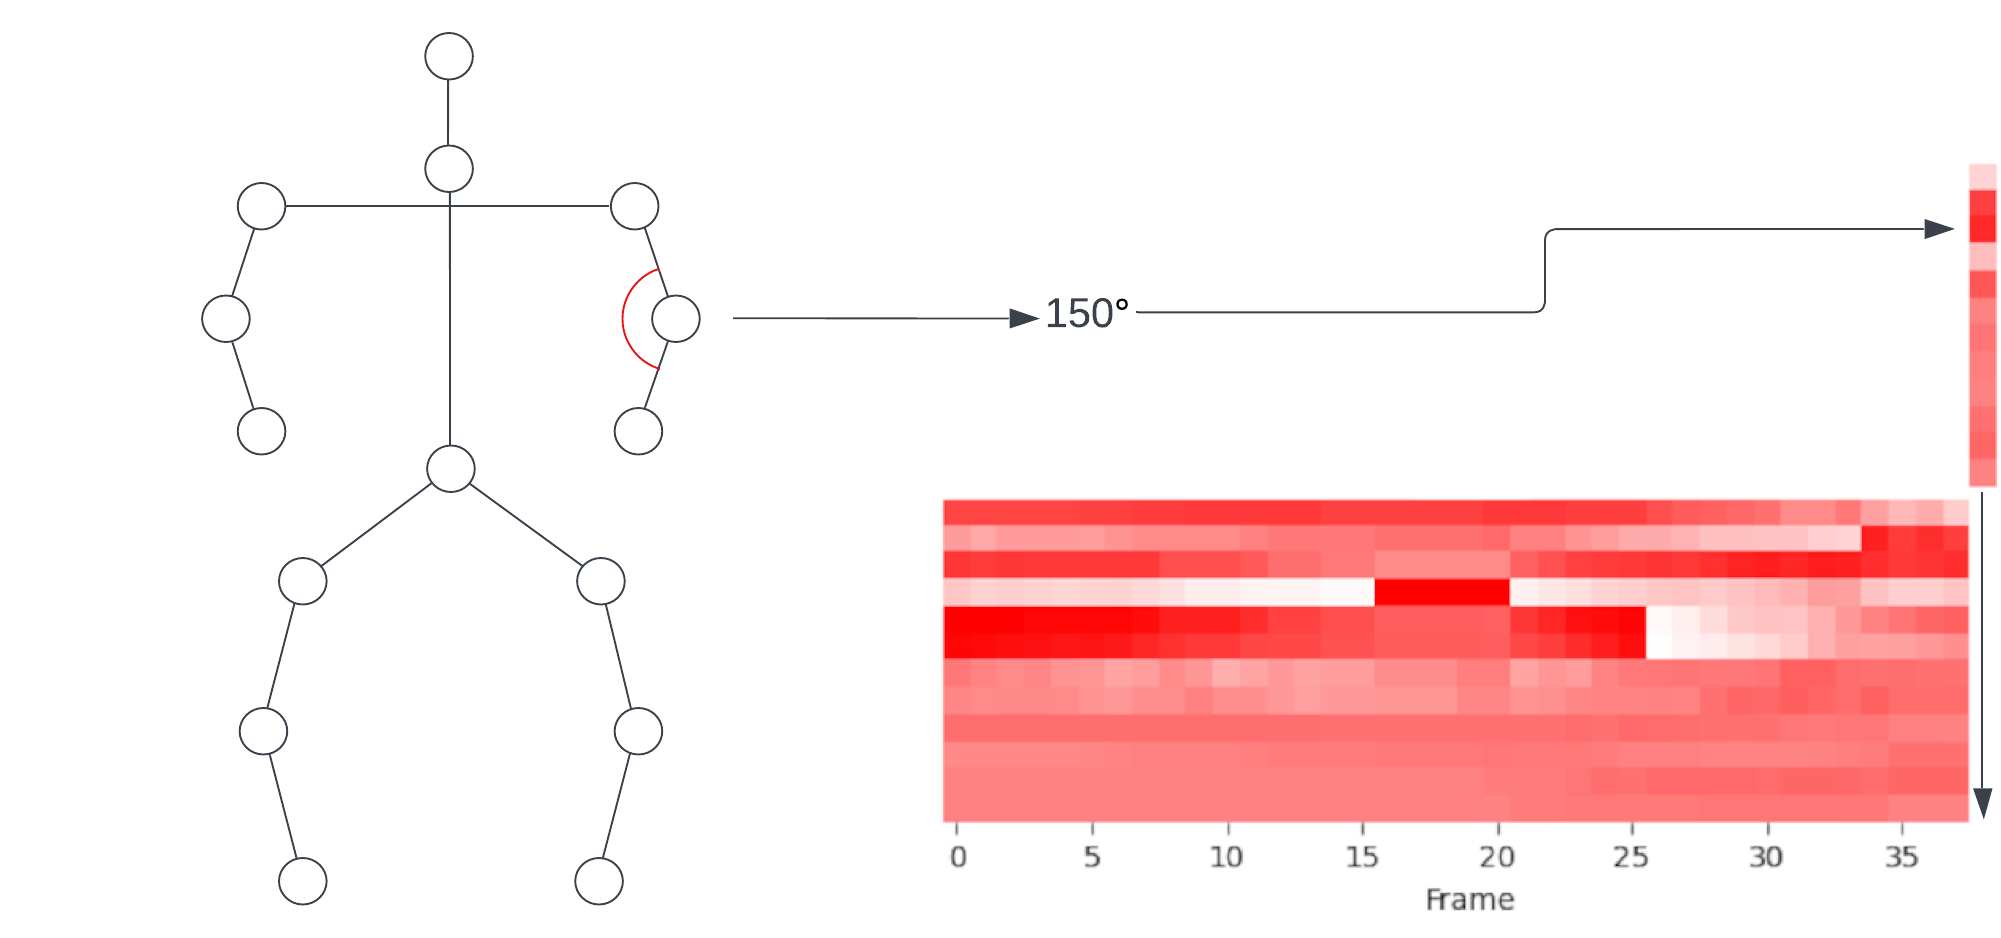
\includegraphics[width=0.6\textwidth]{IntermediateConstruction}}
	\centering
	\caption{Comparison of our representation (b) compared to \textbf{Simple yet efficient real-time pose-based action recognition} \cite{simple_yet_efficient} (a), showing a similar representation construction.}
	\label{fig:simple-v-ours}
\end{figure}

\iffalse
\begin{figure}[ht]
	\subfigure[]{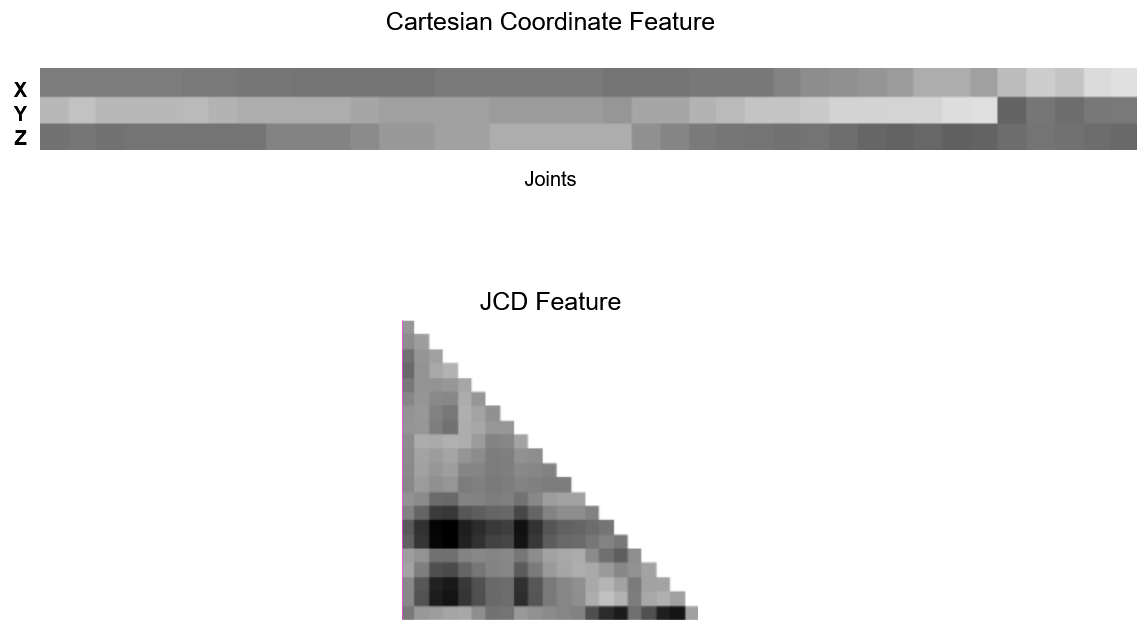
\includegraphics[width=0.6\textwidth]{smallerfasterbetterv2}}
	\subfigure[]{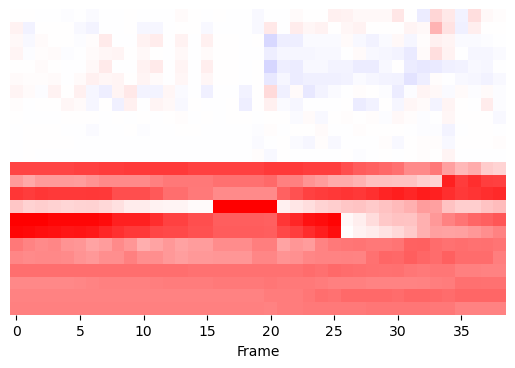
\includegraphics[width=0.6\textwidth]{IntermediateStacked}}
	\centering
	\caption{Similar representations of our novel representation (b) compared to that of \textbf{Make Skeleton-based Action Recognition Model Smaller, Faster and Better} \cite{smaller_faster_better} (a).}
	\label{fig:smaller-v-ours}
\end{figure}
\fi

\textbf{Make Skeleton-based Action Recognition Model Smaller, Faster and Better} \cite{smaller_faster_better} also contains a similar representation to ours. Their representation is broken into two parts: a cartesian coordinate feature and a JCD (Joint Collection Distances) feature. The cartesian coordinate feature is no different to that proposed in other representations \cite{simple_yet_efficient}, suffering from the same background interference. Their JCD feature is similar to ours in that it is only using the pose data, and resistant to background interference. Our representation differs in that rather than using both global and pose data, we restrict to only the pose data to completely eliminate background interference.

\begin{figure}[ht]
	\subfigure[N=0]{
		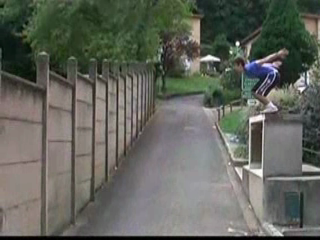
\includegraphics[width=0.2\textwidth]{GolfFrames/D/00012.png}
		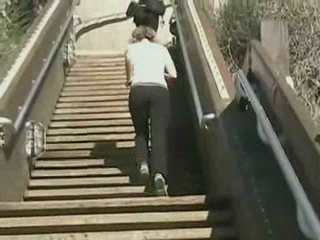
\includegraphics[width=0.2\textwidth]{GolfFrames/D/00013.png}
		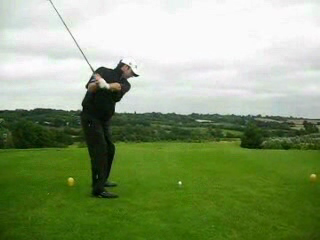
\includegraphics[width=0.2\textwidth]{GolfFrames/D/00014.png}
		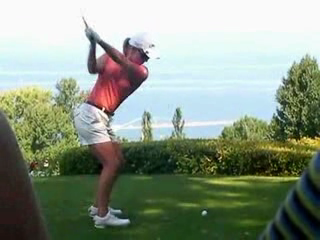
\includegraphics[width=0.2\textwidth]{GolfFrames/D/00015.png}
		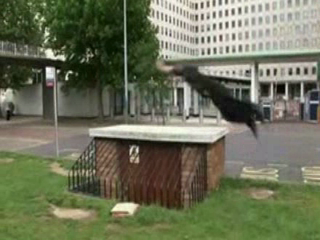
\includegraphics[width=0.2\textwidth]{GolfFrames/D/00016.png}
	}
	\subfigure[N=1]{
		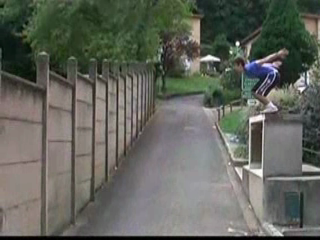
\includegraphics[width=0.2\textwidth]{GolfFrames/D/00012.png}
		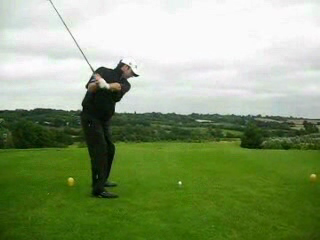
\includegraphics[width=0.2\textwidth]{GolfFrames/D/00014.png}
		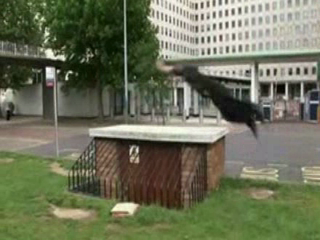
\includegraphics[width=0.2\textwidth]{GolfFrames/D/00016.png}
		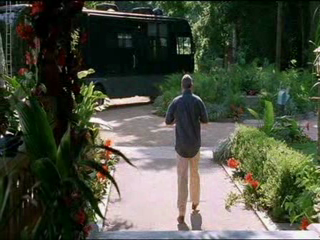
\includegraphics[width=0.2\textwidth]{GolfFrames/D/00018.png}
		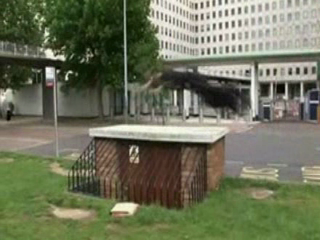
\includegraphics[width=0.2\textwidth]{GolfFrames/D/00020.png}
	}
	\subfigure[N=2]{
		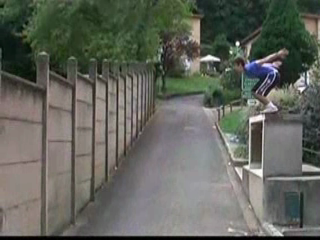
\includegraphics[width=0.2\textwidth]{GolfFrames/D/00012.png}
		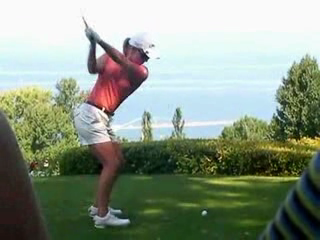
\includegraphics[width=0.2\textwidth]{GolfFrames/D/00015.png}
		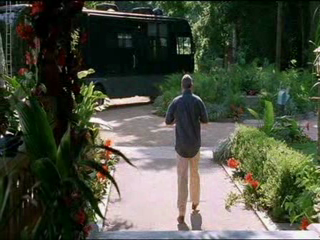
\includegraphics[width=0.2\textwidth]{GolfFrames/D/00018.png}
		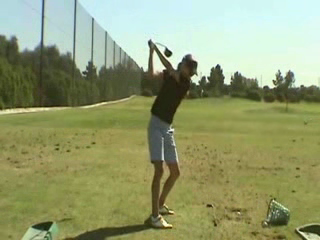
\includegraphics[width=0.2\textwidth]{GolfFrames/D/00021.png}
		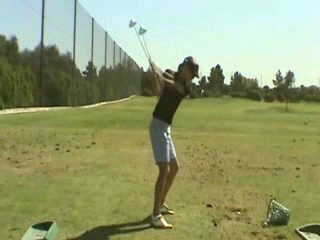
\includegraphics[width=0.2\textwidth]{GolfFrames/D/00024.png}
	}
	\subfigure[N=3]{
		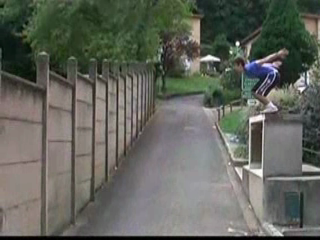
\includegraphics[width=0.2\textwidth]{GolfFrames/D/00012.png}
		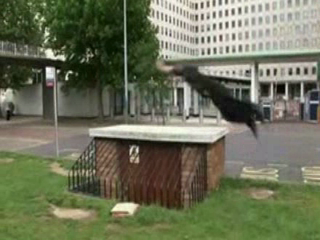
\includegraphics[width=0.2\textwidth]{GolfFrames/D/00016.png}
		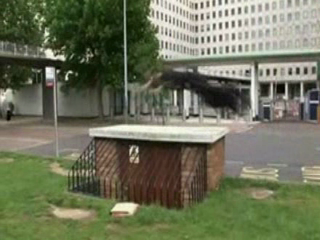
\includegraphics[width=0.2\textwidth]{GolfFrames/D/00020.png}
		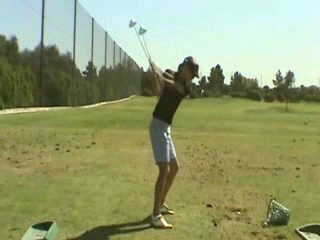
\includegraphics[width=0.2\textwidth]{GolfFrames/D/00024.png}
		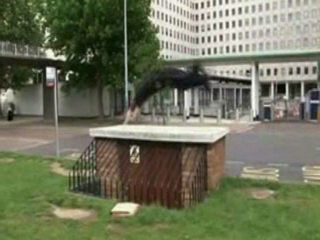
\includegraphics[width=0.2\textwidth]{GolfFrames/D/00028.png}
	}
	\caption{An example of the temporal adjustment on the golf action, skipping N frames between each image. As can be seen in \textbf{(a)}, the movement is not as pronounced and the model may have difficulty determining the action because the velocity of the person is not very pronounced. When observing examples \textbf{(c)} and \textbf{(d)}, the full action from one frame to another is much more clear and the deciphering of the intermediate representation would be easier as the movement is more pronounced.}
	\label{fig:temporal-adjustment-example}
\end{figure}

\subsection{Temporal Adjustments}

It is not unreasonable to assume that moving from only one frame to the next would result in some actions not being represented as well as other actions (this is shown in figure \ref{fig:temporal-adjustment-example}). Due to this issue, we add a temporal adjustment to our representation in order to better represent some of these actions. This is done by adding more channels to the data, with each of the channels "skipping" frames. This would mean that rather than having the angle difference representation moving from frames $1 \rightarrow 2 \rightarrow 3$, in the first additional channel it would move from frames $1 \rightarrow 3 \rightarrow 5$. The representation is then padded out to fit the same shape and added as another channel to the data. This is more clearly shown in figure \ref{fig:intermediate-stacked-skip} where the actions become more "compressed" and movements over longer periods of time become easier to visualize and process.

\begin{figure}[ht]
	\subfigure[N=1]{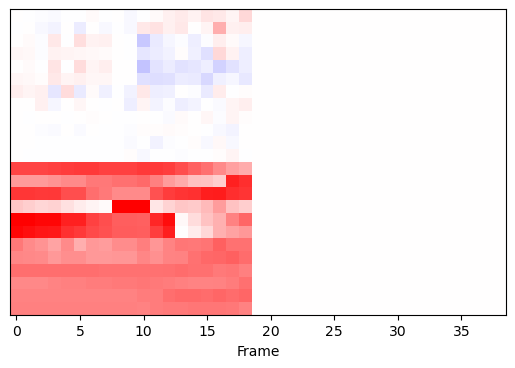
\includegraphics[width=0.4\textwidth]{IntermediateSkip1}}
	\subfigure[N=2]{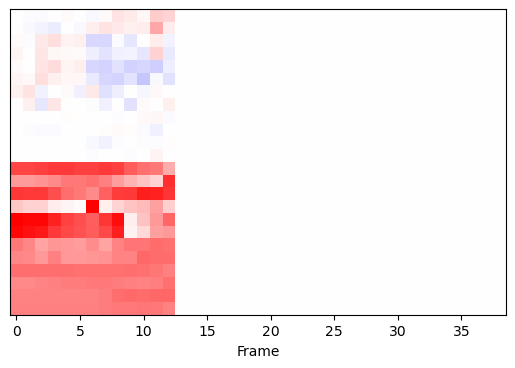
\includegraphics[width=0.4\textwidth]{IntermediateSkip2}}
	\centering
	\caption{Two examples of temporal adjustment to the stacked representation. In both cases, the representation skips N frames in each step, meaning with a $N = 1$ the representation will ignore every other frame, $N = 2$ every two frames, etc. As can be seen from the joint velocities, with example \textbf{(b)}, the joint velocities are more intense and concentrated.}
	\label{fig:intermediate-stacked-skip}
\end{figure}

\subsection{Model Architecture}

The goal of this intermediate representation is to be able to use a simple 2-dimensional CNN which is able to run on simpler and less expensive hardware. The simplified architecture diagram in figure \ref{fig:model-architecture} shows the simple CNN architecture that is to be used. The model consists of 3 convolutional layer groups, followed by global average pooling and the final classification layer. Each individual layer and a more detailed breakdown is shown in table \ref{tab:detailed-model}. 

\begin{figure}[ht]
	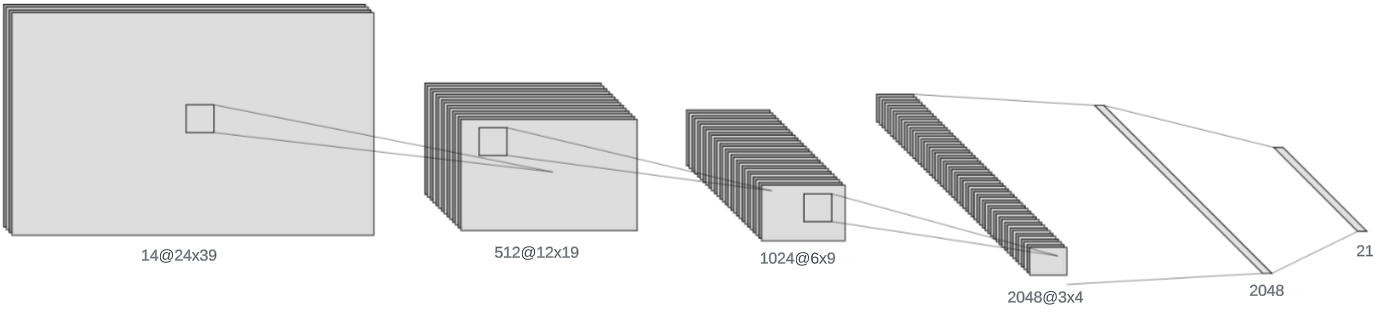
\includegraphics[width=12cm]{ModelArchitecture}
	\centering
	\caption{The basic model architecture used, very similar to that used in other models such as Potion \cite{potion}, it is a simple 2 dimensional CNN that contains one fully connected layer at the end for classification.}
	\label{fig:model-architecture}
\end{figure}

This network is similar to the VGG-16 model previously discussed in section \ref{sec:CNNs} and seen in figure \ref{fig:vgg16}, which is a proven image classification model. Because of the nature of the created intermediate representation, the task can be shifted from processing video to a more classical task of image classification.

\begin{table}[ht]
	\centering
	\begin{tabular}{||c||}
		\hline
		2D Convolution @ 512 Channels \\
		2D Batch Normalization \\
		ReLU \\
		2D Convolution @ 512 Channels \\
		2D Batch Normalization \\
		ReLU \\
		2D Max Pooling\\
		\hline\hline
		50\% Dropout \\
		2D Convolution @ 1024 Channels \\
		2D Batch Normalization \\
		ReLU \\
		2D Convolution @ 1024 Channels \\
		2D Batch Normalization \\
		ReLU \\
		2D Max Pooling\\
		\hline\hline
		50\% Dropout \\
		2D Convolution @ 2048 Channels \\
		2D Batch Normalization \\
		ReLU \\
		2D Convolution @ 2048 Channels \\
		2D Batch Normalization \\
		ReLU \\
		2D Max Pooling\\
		\hline\hline
		Global Average Pooling \\
		Flatten \\
		21 Class Softmax Layer \\
		\hline
	\end{tabular}
	\caption{The detailed breakdown of the model architecture, split into 3 convolutional blocks and one dense layer used for classification. All convolutional layers utilize 3x3 convolutions, including a 1 pixel padding across all sides. The 2D max pooling utilized a 2x2 kernel, halving the size of the images after each convolutional block.}
	\label{tab:detailed-model}
\end{table}

Figure \ref{fig:block-diagram} shows the overview of the model from RGB frames to output. This diagram demonstrates the full pipeline and the overall simplicity of our approach. As has been stated previously in this thesis, the pose estimation model is not fully explored in combination with our model, however when considering an in-the-wild approach it is an important part of the pipeline. This could be similar to the previously discussed OpenPose \cite{openpose} model as discussed in section \ref{sec:pose-detection}, or a much lighter model that can be run on less modern or mobile hardware.

\begin{figure}[ht]
	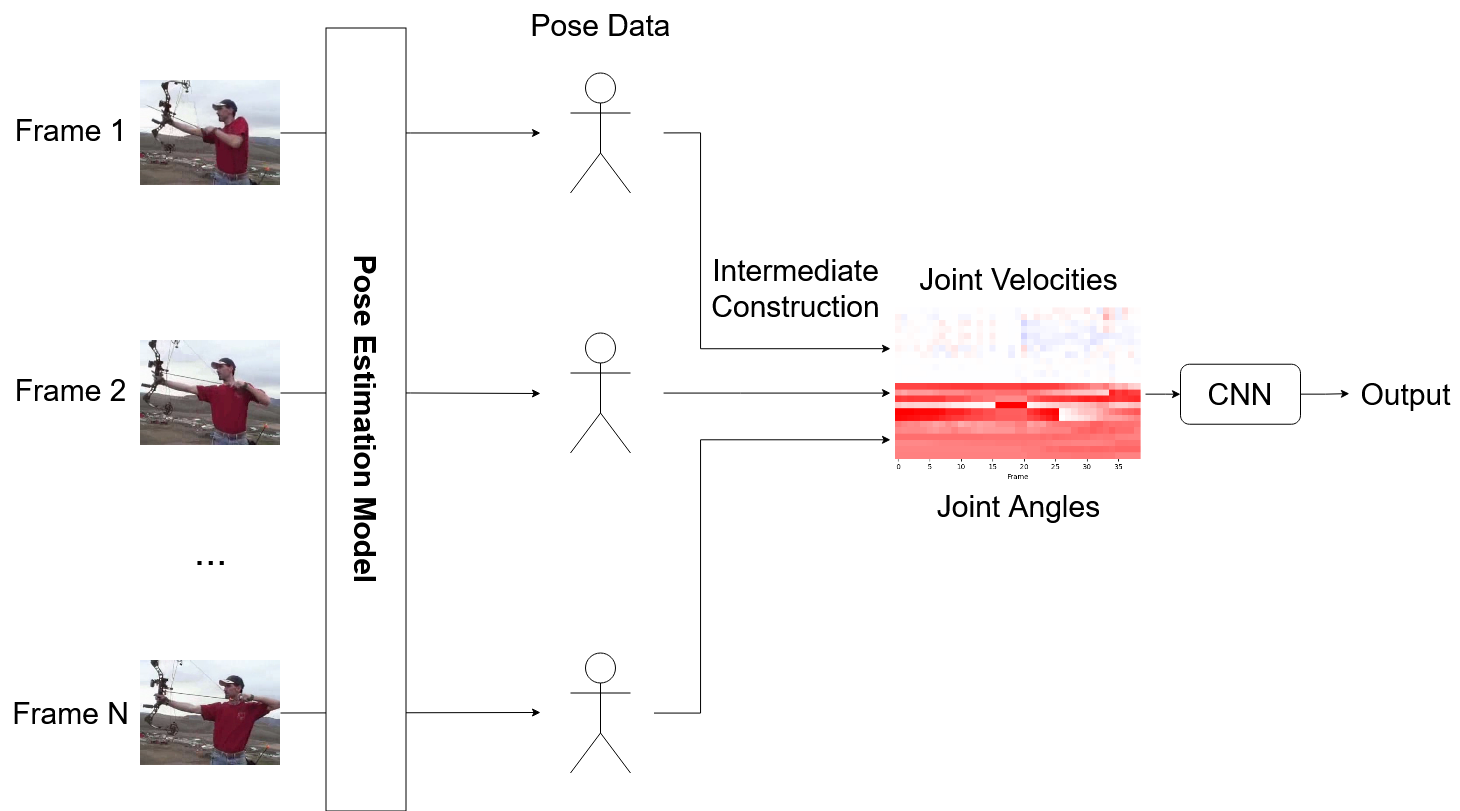
\includegraphics[width=\textwidth]{blockdiagramv2}
	\centering
	\caption{Block diagram showing our intermediate representation from start to finish, including the pose estimation model that was not explored in this thesis.}
	\label{fig:block-diagram}
\end{figure}

This model architecture is very similar to that used in similar papers that construct these intermediate representations. These models have near identical structures to both each other and our proposed end model, with several convolutional layers, followed by a global average pooling, and finally dense layers. As has been stated before, this structure is a classical image classification architecture similar to that of VGG-16 \cite{vgg16}, which is a proven effective model in the image classification task. Our model differs slightly in that it contains more filters than the similar models. While we explored models similar to that used in similar approaches, it was found that using significantly more filters in the convolutions lead to a very large increase in performance, so lower amounts of filters were abandoned in favour of the more complex model.

The model was trained using the stochastic gradient descent (SGD) optimizer, with an initial learning rate of $0.01$, momentum of $0.9$, batch size $16$, and weight decay $0.005$. After each epoch, the learning rate was multiplied by $0.999$, reducing the learning rate gradually over the training period. As the dataset was well balanced with the training and testing datasets and the classes had an even number of examples, the only augmentation was a shuffle operation before each epoch.